\documentclass{article}


% This is now the recommended way for checking for PDFLaTeX:
\usepackage{ifpdf}

% Use utf-8 encoding for foreign characters
\usepackage[utf8]{inputenc}

% Swedish grammar
\usepackage[swedish]{babel}

% Setup for fullpage use
%\usepackage{fullpage}

\usepackage[a4paper]{geometry}

% Space between paragraphs instead of indentation.
\usepackage{parskip}

\ifpdf
\usepackage[pdftex]{graphicx}
\else
\usepackage{graphicx}
\fi

\ifpdf
\DeclareGraphicsExtensions{.pdf, .jpg, .tif, .png}
\else
\DeclareGraphicsExtensions{.eps, .jpg}
\fi

\usepackage{float}

\pdfpxdimen=1in
\divide\pdfpxdimen by 300

%\footskip=1in
%\voffset=1in

\title{
  Projekt iMalloc \\
  Imperativ och objektorienterad programmeringsmetodik, 1DL221
}
\author{
  Niclas Edenvin \\
  Åke Lagercrantz \\
  Andreas Lelli \\
  Daniel Lindgren \\
  Elias Lundeqvist \\
  Jakob Sennerby
}

\date{2012-11-09}



\begin{document}

\maketitle

\vspace{4cm}

\begin{abstract}
  \centering
  \begin{minipage}{0.75\textwidth}
  { 
  \parskip5pt

  \noindent Vi fick i uppgift att, i programmeringsspråket c, konstruera ett eget bibliotek för minneshantering.

  \noindent  Genom att dela upp uppgiften i mindre block och följa projektspecifikationen skapade vi en minneshanterare med flera alternativ för hur man vill behandla minnet.

  \noindent  Problemet löstes enligt specifikationerna och resultatet blev som väntat en effektiv minnesallokerare som med fördel kan användas av program som vill kunna bestämma själv på vilket sätt minnet ska användas.
  }

  \end{minipage}


\end{abstract}


\newpage

\tableofcontents

\newpage

% *********************
% Infoga bild

% se Figur \ref{fig:stable}.

%\begin{figure}[H]
%  \includegraphics[width=165mm]{stabil.png}
%  \caption{Den slutliga versionen av kretsen i Logisim.}
%  \label{fig:stable}
%\end{figure}


% *************************************************************************
% *************************************************************************
% *************************************************************************
% *************************************************************************
\section{Dagbok}

\subsection{Fredag 19 Oktober}

Vi träffades hemma hos Niclas för att gemensamt gå igenom instruktionerna och förbereda oss för första projektveckan. Vi bestämde även att vi skulle använda oss av olika applikationer, tjänster och versionshanteringssystem som gör det enklare för oss att arbeta tillsammans samt hålla koll på hur vårt arbetsflöde fungerar. Vi valde att använda oss av

\begin{description} \parskip0pt
  \item[Git och github] versionshanteringssystem
  \item[Trello] strukturering av uppgifter och vem som gör vad
  \item[Tickspot] tidsrapportering
  \item[Hipchat] kommunikation och forum
  \item[Google Drive] utkast av projektdagbok och övriga dokument
\end{description}
Vi började även skissa på en övergripande design för systemet för att hitta en lämplig uppdelning.

\subsection{Måndag 22 Oktober}

Vi gjorde klart den övergripande designen. Se Figur \ref{fig:design}. Sedan bestämde vi oss för en gemensam kodstandard enligt följande:

\begin{description} \parskip0pt
  \item[Tab size] 2 med soft tabs
  \item[Exempel funktionsnamn] king\_in\_danger
  \item[Exempel variabelnamn] king\_color
\end{description}

Vi delade slumpvis in oss i par och tilldelade paren varsin del av programmet och började sedan jobba i paren med headerfilerna.

{\bf Andreas och Daniel} Den större delen av dagen gick åt till att planera hur projektet skulle vara utformat. Vi började arbeta på skräpsamlingen och test för dessa.

{\bf Elias och Jakob} Gick igenom hur minneshanteringen kommer fungera på representationsnivå. Diskuterade en del med Åke och Niclas också och kommer inte fram till någon vettig lösning. Vi pratade med våran coach Niklas också och han sa att han inte har fått tillräckligt med info för att hjälpa oss med detta. Vi mailar Tobias för att se vad han har att säga.

{\bf Niclas och Åke} Gjorde makefile och skelett till unittesting. Försökte lösa designproblemet med hur refcount och de privata managed- och manualobjekten ska hanteras.


\begin{figure}[H]
  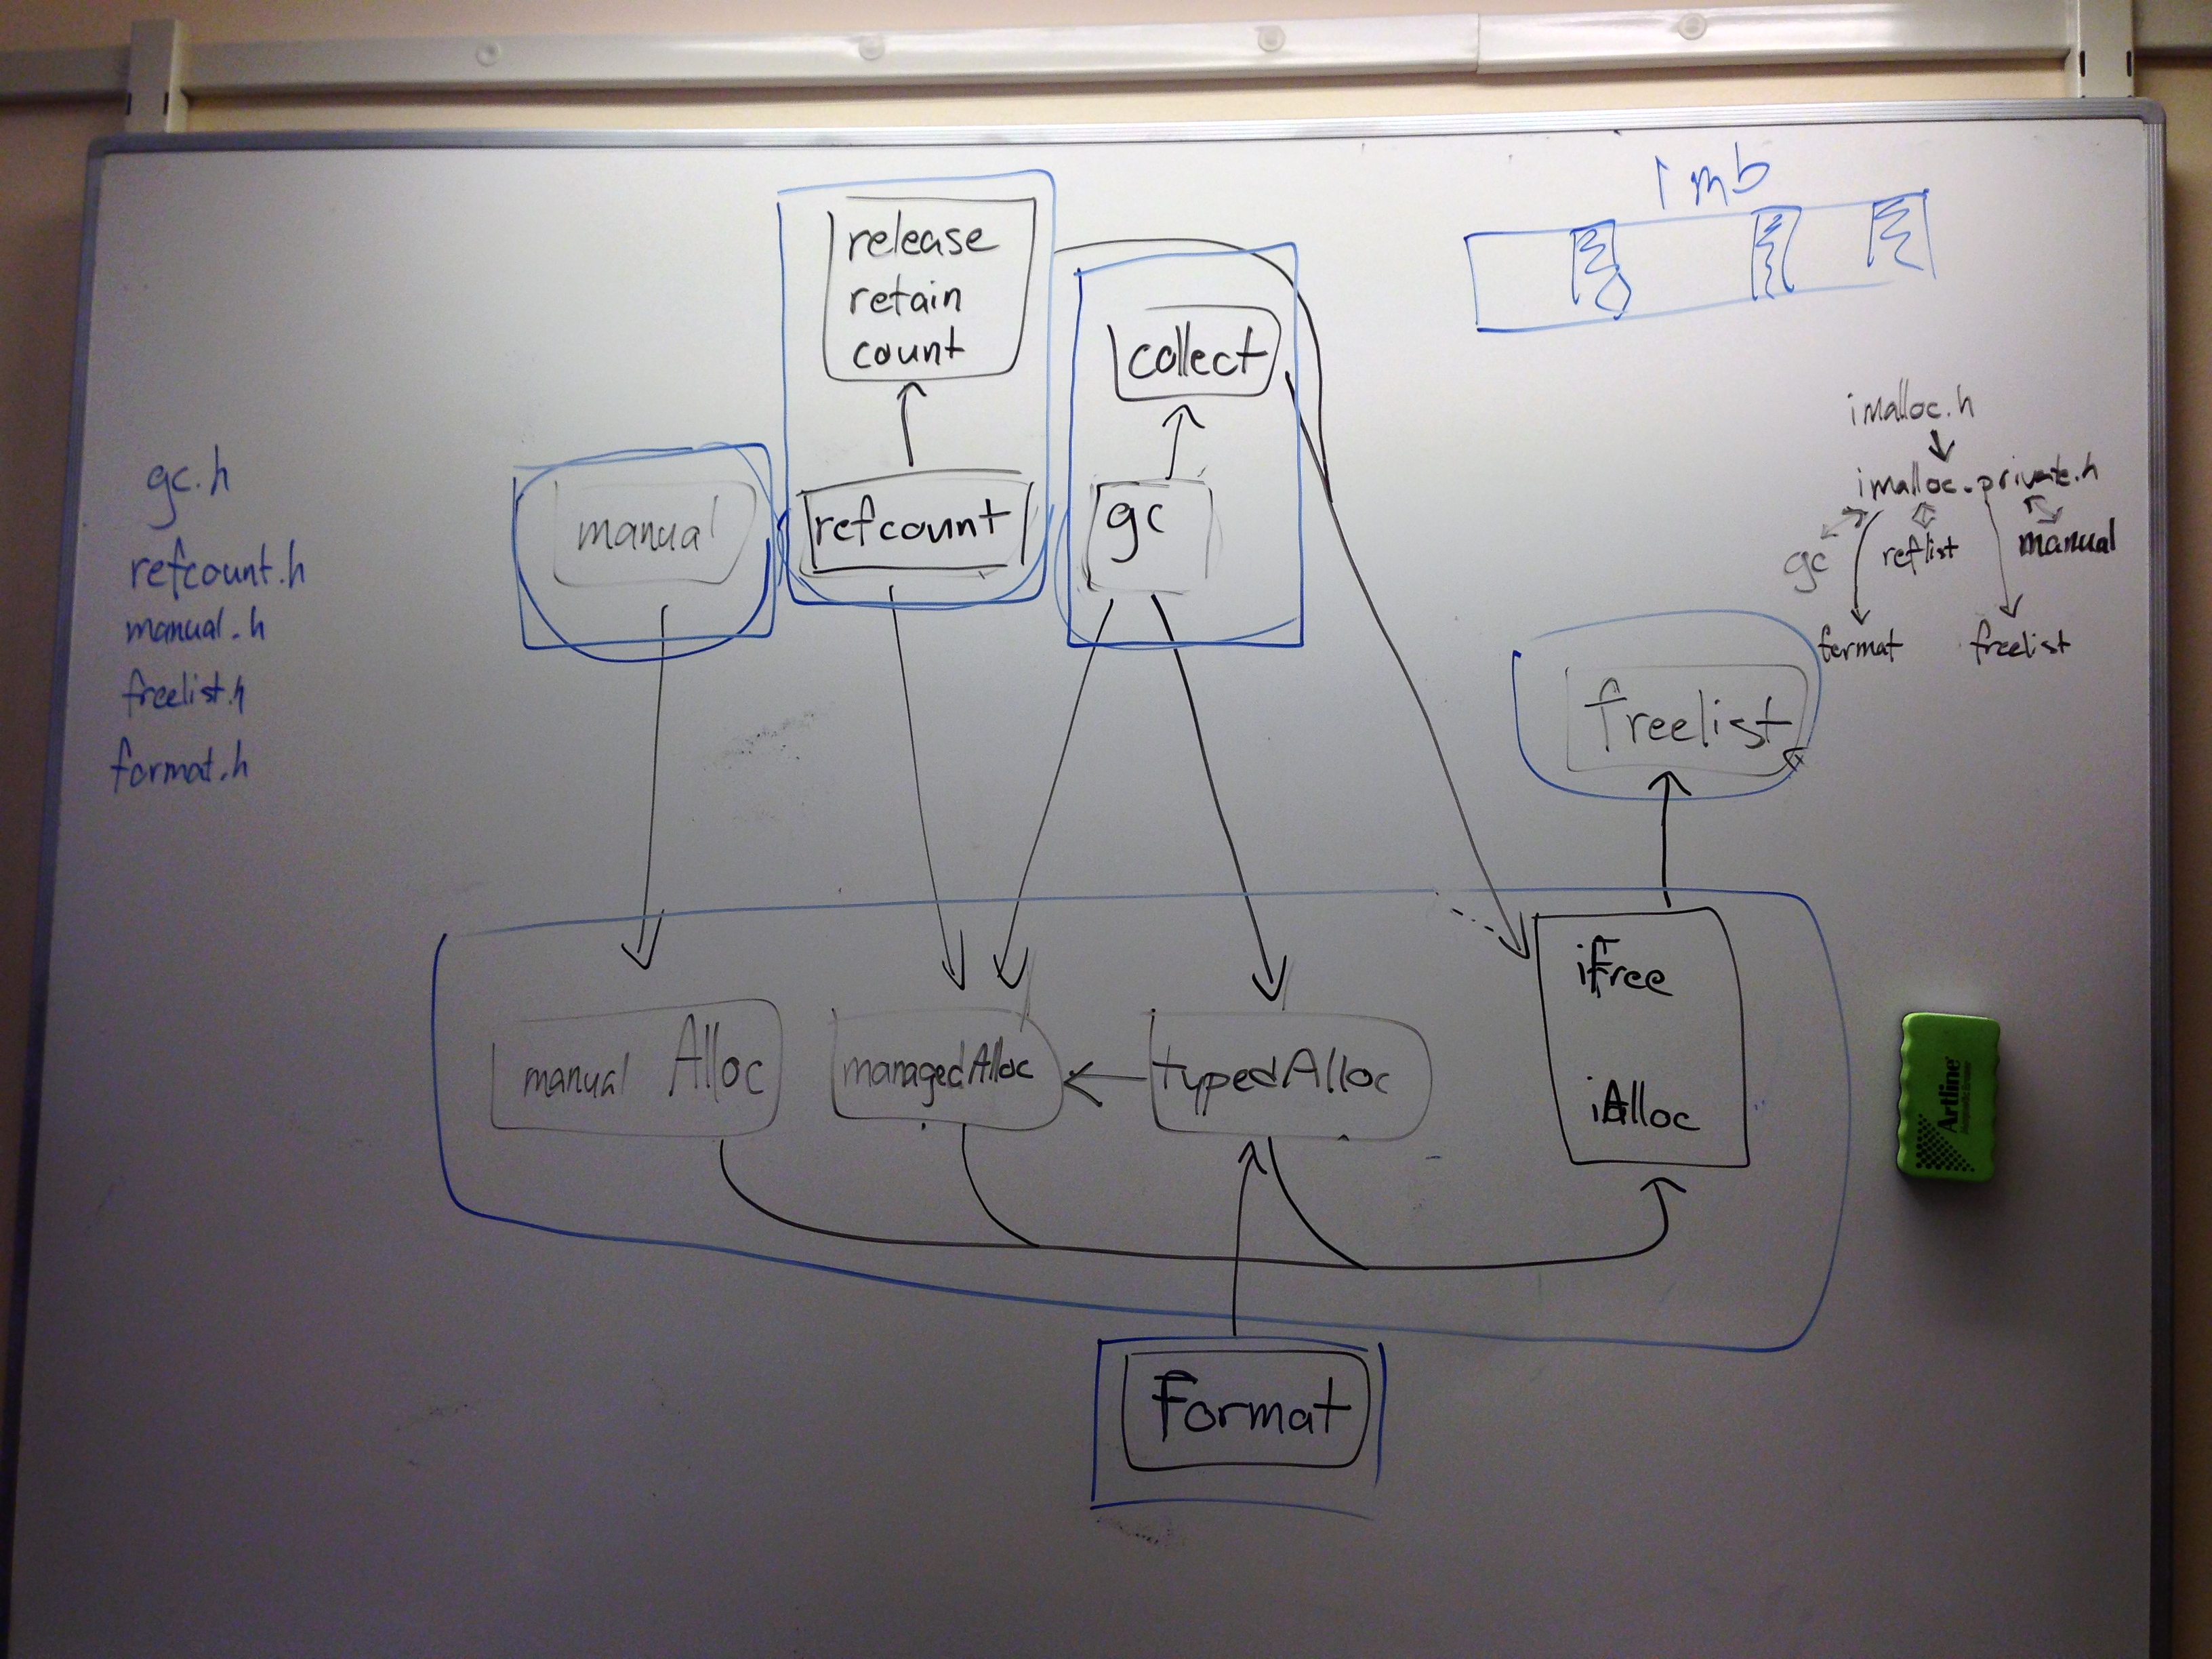
\includegraphics[width=\columnwidth]{../bilder/design_whiteboard.jpg}
  \caption{Våran ursprungliga design och indelning.}
  \label{fig:design}
\end{figure}

\subsection{Tisdag 23 Oktober}

{\bf Andreas och Daniel} Vi fortsatte arbeta på gc och diskuterat på vilket sätt den borde fungera. Koden för att traversera stacken har inte delats ut ännu, av denna anledning är det svårt att få våra testfall att fungera som de bör (Då vi ej kan traversera stacken på ett vettigt sätt utan att se vilka pekare som leder dit).

{\bf Elias och Jakob} Vi satt fast och kunde inte riktigt koda någonting på grund av att vi inte visste hur vi skulle representera våran freelist, alloclist och refcount. Vi väntade på svar från Tobias men började koda på formatstring så länge.

Vi blev klara med formatstring och alla tester till denna innan samtliga i gruppen gick och pratade med Justin Pearsson. Justin berättade att vi skulle “gömma” freelist och alloclist innan stylen och även refcount skulle “gömmas” innan objektet. Vi började arbeta med refcount igen och gjorde klart det mesta förutom release-delen. Vi kunde inte riktigt arbeta mer då vi behöver färdig kod för “ifree”. Därför har nu release och testkoden en del placeholders.

{\bf Niclas och Åke} Fortsatte på funktioner i memory. Fixade unittests så att alla kan skriva tester. Tillämpade TDD och par-switching (highfive!). Vi gick även och pratade med Justin som tyckte att det var helt ok att göra som vi tänkt att spara refcount direkt innan varje objekt på heapen, trots att programmeraren då förlorar en del minne.


\subsection{Onsdag 24 Oktober}
{\bf Andreas och Daniel} Idag arbetade vi med gc.c och främst funktioner för traversering och markering av element på heapen. Vi fastnade en del på hur vi skulle göra med de element på heapen som var en pekare till andra element inom adressrymden, i början valde vi att spara allt på en lista och sedan markera dem en och en men ändrade oss sedan till att använda rekursion. Vi är snart även klara med Sweep-delen av algoritmen, dvs den delen då vi friar upp de objekt som inte har blivit markerade som använda.

{\bf Jakob och Elias} Eftersom vi inte kan slutföra refcount på grund av att release inte har funktioner tillräckligt för att free:a korrekt så har vi nästan gjort färdigt priv\_imalloc idag, det saknas lite tester. Efter två timmars diskuterade om hur exemplen som finns i projektspecen var tänkt att fungera så gick vi och Åke till Wrigstad och fick konstaterat för oss att det var som vi trodde, dvs fel i specen.

{\bf Niclas och Åke} Vi fortsatte på funktioner och tester av memory. Vi försökte också komma på hur vi ska göra med cross-referencing som vi har på vissa ställen.

\subsection{Torsdag 25 Oktober}

{\bf Andreas och Daniel} Idag har vi arbetat en hel del på funktionerna för att traversera heapen, Swipe algoritmen och markeringsalgoritmen. Vi har fått det mesta att fungera och börjat felsöka. Vi behöver dock funktionen för att traversera Stacken innan vi kan säga att GC är helt klar men det borde inte vara mycket arbete kvar här nu!

{\bf Jakob och Elias} Har jobbat med priv\_imalloc för det mesta idag. Det har gått bra. Vi är nästan färdig med implementationen av själva imalloc-funktionen. Har mest felsökning kvar. Sedan kan vi förhoppningsvis börja med priv\_free (a.k.a ifree) så vi kan slutföra refcount.


{\bf Niclas och Åke} Arbetat med tester och funktioner i memory. Löst problemet med cross-referencing av headerfiler. Designändringar i vissa structs gällande memory. Implementerat en privat headerfil för memory, så att vi kan testa våra privata hjälpfunktioner med enhetstestning.

\subsection{Fredag 26 Oktober}

{\bf Andreas och Daniel} Vi har först och främst gjort klart GC, vi har implementerat funktionerna för att traversera stacken och allting kompilerar som det sig borde. Vi måste dock fixa våra testfall då dessa inte längre fungerar på grund av att vi har ändrat hur minnet beter sig. Dessutom kräver testerna (för att kunna testa vettiga saker) att iMalloc är mer eller mindre klar, detta eftersom att gc ska “städa undan” data genererad av användaren. Vi har kollat på olika program för koddokumentation och de bäst lämpade tycks vara Doxygen som vi började arbeta med då det kan generera latexkod. Vi har även hunnit göra två stycken “flow charts” för hur de olika modulerna kommunicerar med varandra.

{\bf Jakob och Elias} Precis som igår arbetade vi idag med priv\_imalloc, vi skrev klart alla funktioner samt skrev tester som vi tidigare inte kunnat skriva pga. de okompletta memory-funktionerna. Nu återstår bara en del småfix och felsökning.

{\bf Niclas och Åke} Implementerat memory\_claim och diverse underfunktioner. Tester för desamma. Memory känns nu mer eller mindre klart, finns en del småfix och felsökning att genomföra.

\subsection{Måndag 29 Oktober}
{\bf Samtliga} Idag träffade vi vår coach Niklas för ett avstämningsmöte. Vi roterade även parkombinationerna och under den här veckan kommer följande par att arbeta:

\begin{description} \parskip0pt
  \item[Andreas och Niclas] Dokumentation
  \item[Jakob och Åke] priv\_imalloc
  \item[Daniel och Elias] garbage collection
\end{description}

Arbetsfördelningen kommer att variera en del under veckan då de flesta av våra funktioner är mer eller mindre färdiga.

{\bf Andreas och Niclas} Vi började under dagen bygga upp all dokumentation som ska in. Vi har helt enkelt börjat sammanställa all tidsrapportering, alla övergripande designdokument etc och sammanställt detta till en inlämningsbar rapport.

{\bf Elias och Daniel} Idag har vi jobbat med gc-delen, det blev vi som fick fortsätta med den efter rotationen. Elias fick lite tid att sätta sig in i koden och efter det släppte Jakob och Åke ut ny kod till priv\_imalloc. Detta resulterade i att vi fick modifiera vår kod då priv\_imalloc nu hade olika funktioner för managed och manual alloc, något den inte hade tidigare. Detta gjorde att vi fick en del problem att kompilera vår kod. Därefter löste Åke och Jakob lite problem, varpå vi kunde ändra tillbaka vår kod till den ursprungliga. Vi fick koden att fungera som det var tänkt men det saknas fortfarande tester, något vi inte har kunnat göra då vi behöver ha iMalloc helt färdigskriven.

{\bf Jakob och Åke}
Skrev fler tester för priv\_imalloc samt spenderade mycket tid på att debugga kod här och var. Alla började bli typ klara med sina delar och vi försökte sätta ihop och testa dem tillsammans.

\subsection{Tisdag 30 Oktober}

{\bf Andreas och Niclas}
Under dagen arbetade vi en del med koddokumentation men gick sedan över till att bygga upp de dokument vi skall lämna in i Latex. Vi har lagt in dagboken, arbetat på diverse stapeldiagram för att visa tidsfördelningen och under processen även lärt oss hur man arbetar i latex!

{\bf Daniel och Elias}
I väntan på att Åke och Jakob ska bli färdig med priv\_imalloc så har vi börjat skriva på den övergripande designdokumentationen. Vi har haft problem med att förstå vad man ska få med och hur, men vi har skrivit det så bra vi kan utifrån vår tolkning. Efter det kom vi igång med gc:s test igen och satt med det resten av dagen.

{\bf Jakob och Åke}
Skrev klart sista delarna av priv\_imalloc inkl tester. Fortfarande massor av buggar. 32-bitars minnesadresser i traverse\_heap på 64-bitarsmaskiner, varifrån kommer dem?

\subsection{Onsdag 31 Oktober}
{\bf Andreas och Niclas}
Under dagen arbetade vi med de dokument vi skall lämna in, vi har fortsatt formatera allt i Latex, ordnat med graferna och gjort klart den övergripande designen. Vi felsökte också GC tillsammans med de andra grupperna.

{\bf Daniel och Elias}
Idag har vi ägnat all tid åt felsökning av GC. Vi har problem när vårt test för GC:n har skräp att samla.

{\bf Jakob och Åke}
Debuggade gc-delen. Skrev om stora delar av traverse\_heap. Olika problem på olika platformar. BUS error på SPARC, segfaults på x86.

\subsection{Torsdag 1 November}
{\bf Andreas och Niclas} Vi har delvis vart med och diskuterat fel i GC men främst har vi arbetat med koddokumentation på gränssnittsnivå och övriga dokument som skall lämnas in.

{\bf Daniel och Elias} Vi har även idag ägnat all tid åt felsökning i GC. Vi löser fler och fler fel men det dyker alltid upp nya. Har fått mycket hjälp från de andra grupperna då de har ungefär samma problem.

{\bf Jakob och Åke} Fixat massa buggar i gc. Nu stegar vi bla. rätt längd i traverse\_heap oavsett platform.

\subsection{Fredag 2 November}
{\bf Andreas och Niclas} Samma som tidigare dagar, koddokumentation på gränssnittsnivå, finslipning av de dokument vi ska lämna in.

{\bf Daniel och Elias} Debuggande (som hela denna vecka). Sen övergick vi till att skriva på dokumentationen. Elias jobbade främst på reflektionen över grupparbetet medan Daniel började med ett dokument om gränssnitten mellan modulerna.

{\bf Jakob och Åke} Fortsätter med debugging men kommer inte riktigt någonstans. Hittade ett sätt att skriva ut hela stacken i gdb men hjälpte inte så mycket. Nya tag på Måndag!

\subsection{Söndag 4 November}
{\bf Åke} Listade ut var våra "spökpekare" kommer ifrån. De ligger kvar på stacken från tidigare stackframes som återanvänds utan att all data i stackframen skrivs över.

\subsection{Måndag 5 November}
{\bf Andreas och Niclas} Vi har arbetat på koddokumentationen på gränssnittsnivå och mer eller mindre skrivit klart reflektionen. Tillsammans med övriga har vi varit uppe och pratat med Elias Castegren och Justin Pears beträffande de sista problemen vi haft med vår kod.

{\bf Daniel och Elias} Idag har Elias fokuserat främst på att skriva dokumentation och börjar bli klar med de första utkasten nu och ska sedan börja finslipa på allt. Daniel har arbetat med buggarna i GC samt skrivit lite mer på gränsnitten mellan modulerna.

{\bf Åke} Lyckades ta bort många av spökpekarna genom att innan collect anropas rensa stacken ovanför från pekare. En spökpekare återstod dock vid normal körning, men denna försvinner mystiskt när programmet stegas igenom gdb.Detta leder oss till att tro att det kan vara en pekare som ligger i ett register som inte töms. Exprimentering med jmp_buf ledde dock ingen vart. Vi bestämde oss för att anse att problemet inte är så viktigt då pekarna i ett verkligt scenario skulle skrivas över förr eller senare och på så sätt tas bort som skräp. Det är ju bara enhetstesterna som strular på vissa platformar, inte själva koden.

{\bf Jakob} Var bollplank åt Åke.

\subsection{Tisdag 6 November}
{\bf Daniel} Skrev på gränsnitten mellan modulerna.

{\bf Andreas} Arbetade med koddokumentation på gränssnittsnivå och reflektion. Vi pratade även med Tobias efter föreläsningen om vårt problem betr. skräp på stacken. 

{\bf Jakob} Sjuk.

{\bf Niclas} Arbetat på koddokumentationen på gränssnittsnivå.

{\bf Åke} Skrev på reflektion & dokumentation.

{\bf Elias} Skrivit reflektion.

\subsection{Onsdag 7 November}

% *************************************************************************
% *************************************************************************
% *************************************************************************
% *************************************************************************
\section{Parrotationer}
Den första dagen jobbade vi allihopa tillsammans. Vi gick igenom instruktionerna och diskuterade uppgiften. Vi valde att inte dela upp oss i par innan vi var säkra på hur vi ville dela upp uppgiften och hade koll på strukturen.

\subsection{Vecka 1}
Dag två delade in oss i par baserat på den övergripande designen vi hade gjort. Vi använde oss av en slumpgenerator för att ta fram paren samt även vilket par som skulle jobba med vad. Under första veckan jobbade vi så här:

\begin{description} \parskip0pt
  \item[Niclas och Åke] memory
  \item[Elias och Jakob] refcount
  \item[Andreas och Daniel] garbage collection
\end{description}

Detaljerade beskrivningar av koddelarna finns under \ref{sec:design}.

\subsection{Vecka 2}
Vi räknade med att arbetsfördelningen skulle variera under andra veckan då vi var klara med de flesta stora delar. Däremot roterade vi paren slumpmässigt, precis som första veckan. Vi slumpade även vilka som skulle sitta kvar med samma uppgift som tidigare. Gruppindelningen vecka två såg ut så här:

\begin{description} \parskip0pt
  \item[Andreas och Niclas] dokumentation
  \item[Jakob och Åke] priv\_imalloc
  \item[Daniel och Elias] garbage collection
\end{description}

\subsection{Vecka 3}
När vi började vecka 3 var vi i princip klara med all kodskrivning. Därför valde vi att inte jobba i bestämda par, utan vi jobbade mer flytande.


% *************************************************************************
% *************************************************************************
% *************************************************************************
% *************************************************************************
\section{Tidsåtgång}

Under projektets gång har vi arbetat med ett program för “Time Tracking” som heter Tick. Efter varje arbetsdag rapporterade alla in hur många timmar dem hade arbetat samt hur många timmar dem har lagt på diverse delar av projektet.

Vi har totalt arbetat 230 timmar med projektet varav 6 timmar på möten, x timmar på dokumentation, x timmar på planering samt x timmar på implementation och testning.

Då vi har försökt arbeta enligt test driven development är det svårt att räkna ut hur mycket tid som gick specifikt till testerna utan vi ser det som en del av implementationen. Nedan följer två diagram där arbets- och tidsfördelningen är tydlig.

\begin{figure}[H]
  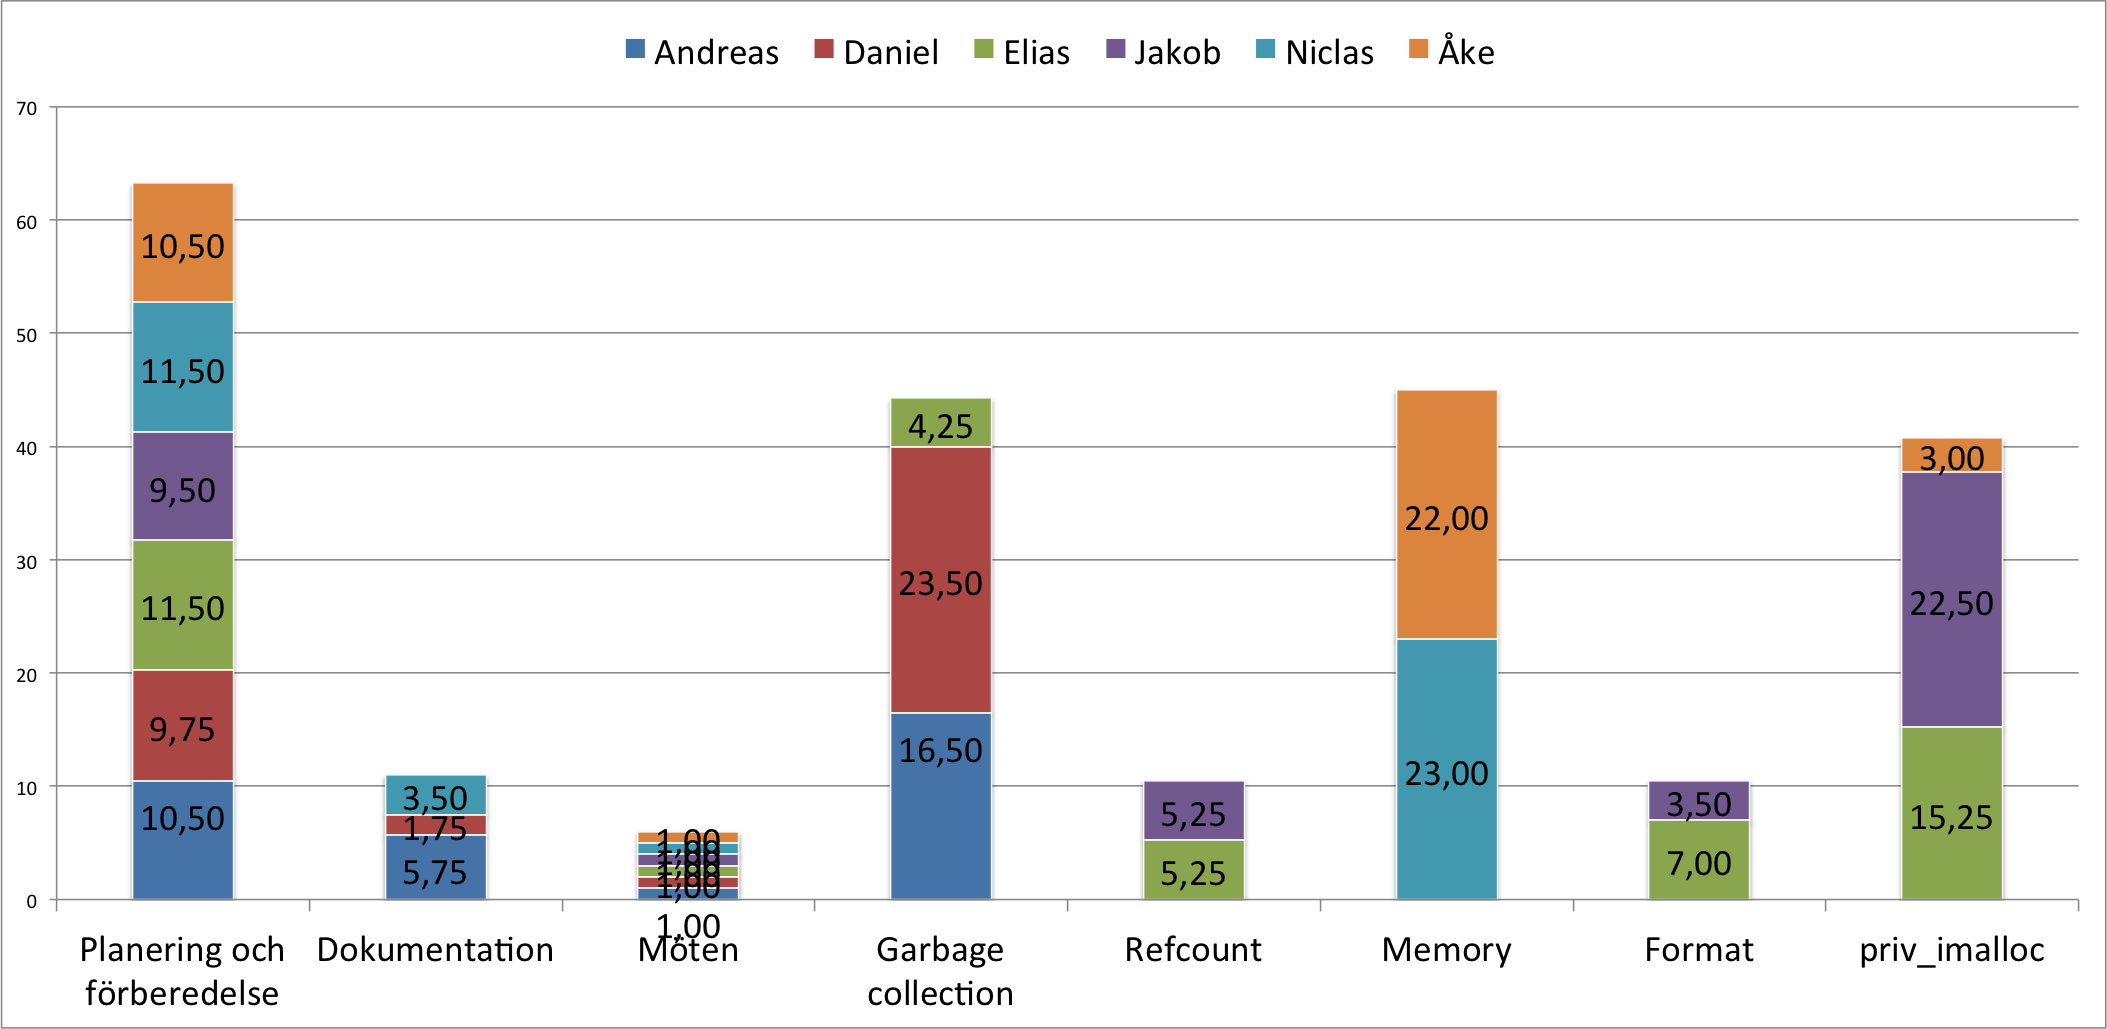
\includegraphics[width=\columnwidth]{../bilder/chart_parts.png}
  \caption{Tidsfördelningen över projektets olika delar 
    samt vem som arbetat på vad.}
  \label{fig:chart_parts}
\end{figure}

\begin{figure}[H]
  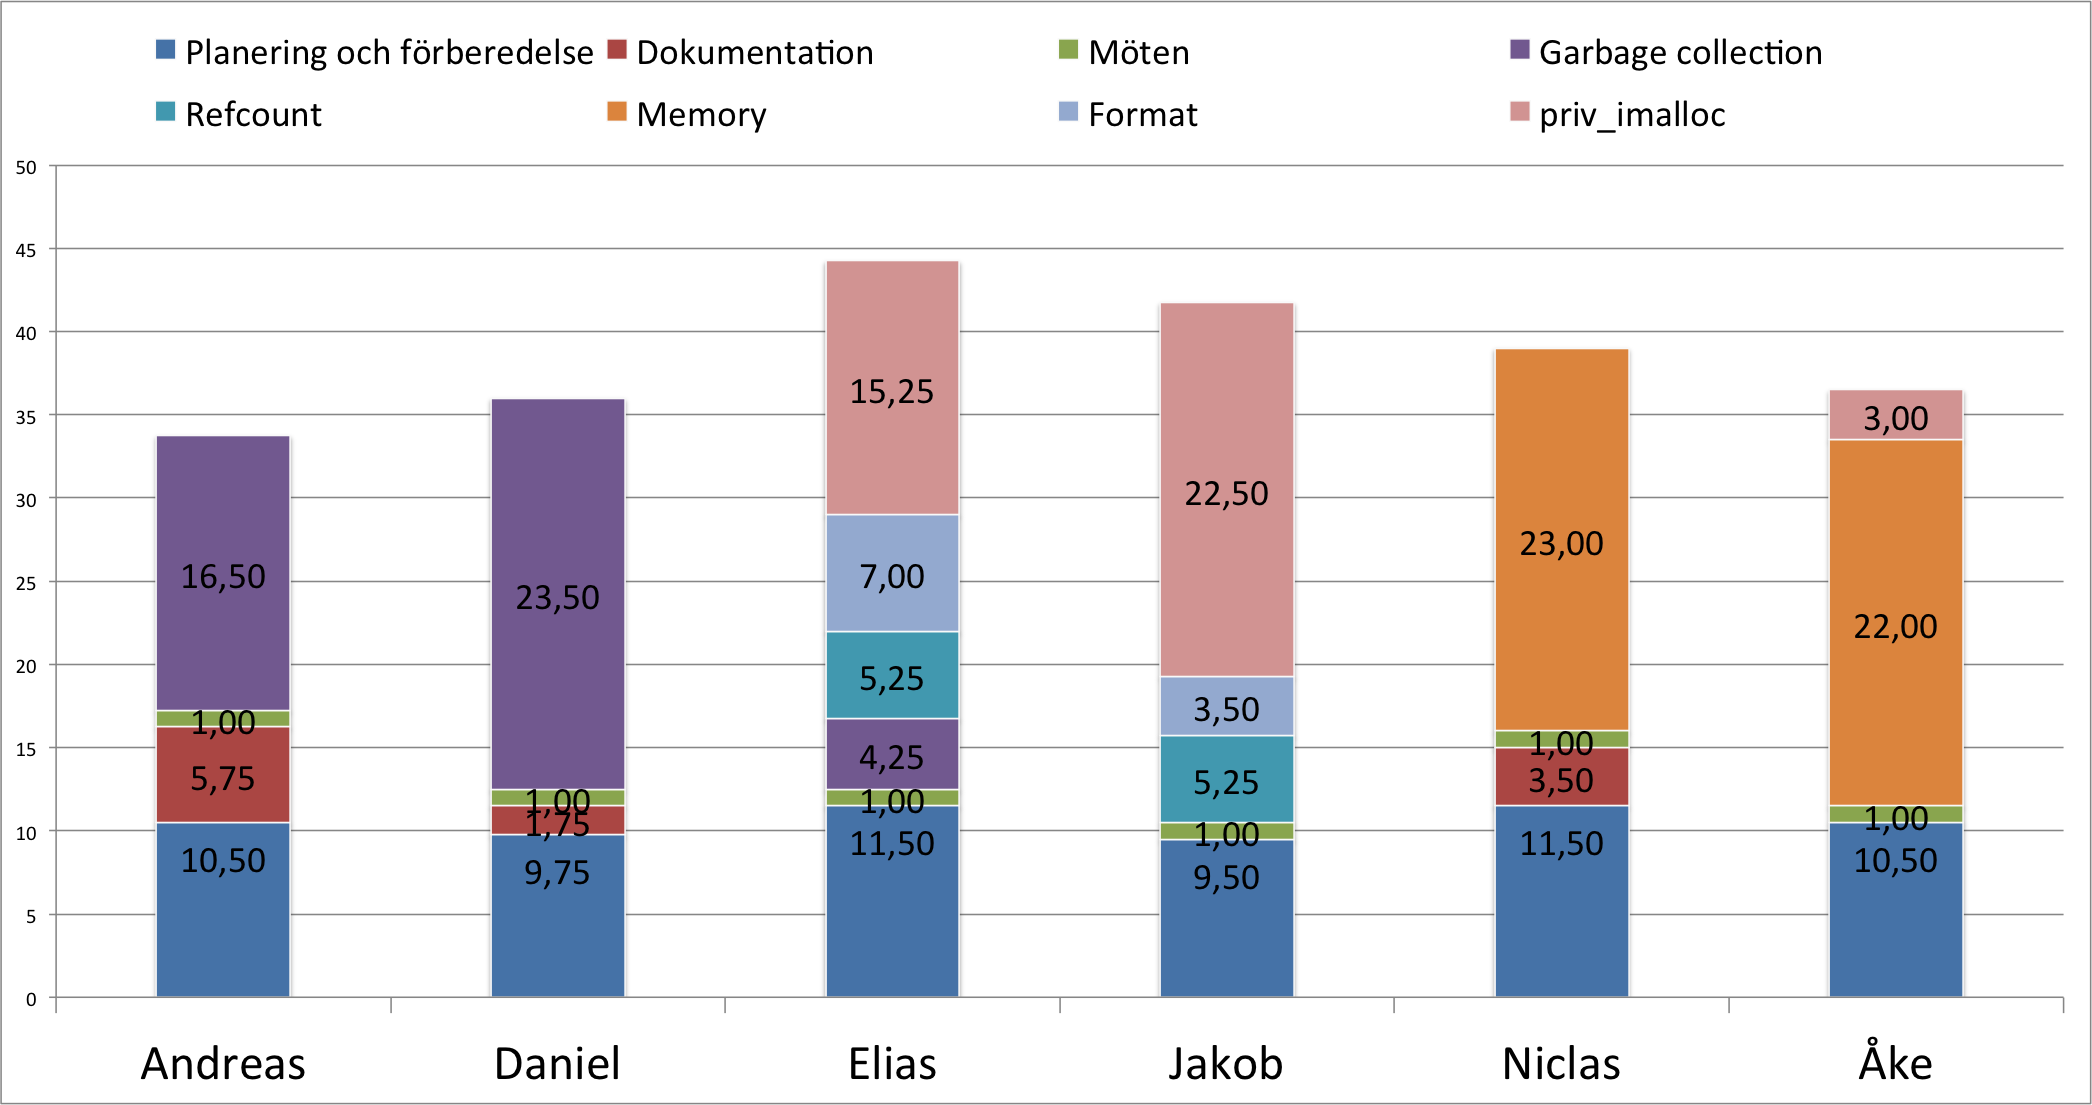
\includegraphics[width=\columnwidth]{../bilder/chart_people.png}
  \caption{Personlig tidsfördelning över de olika delarna av projektet.}
  \label{fig:chart_people}
\end{figure}


% *************************************************************************
% *************************************************************************
% *************************************************************************
% *************************************************************************
\section{Brister}


% *************************************************************************
% *************************************************************************
% *************************************************************************
% *************************************************************************
\section{Bilagor}
\appendix
\section{Övergripande designdokument}
\label{sec:design}
\section{Koddokumentation på gränssnittsnivå}
\section{Gränssnitten mellan modulerna}
\section{Reflektion}



\end{document}

